The first finite difference scheme considered, was the one used by Holden and Raynaud \cite{holden2006convergence}:
\begin{align}
m &= u - D_{-}D_{+}u, \notag \\ 
m_t &= -D_{-}(mu) - mD(u),
\end{align}
where the operators are defined as
\begin{align}
\label{eq:operators}
D_{+}u_{j}^{n} = \frac{u_{j}^{n}-u_{j-1}^{n}}{h},\quad
D_{-}u_{j}^{n} = \frac{u_{j+1}^{n}-u_{j}^{n}}{h},\quad
D = \frac{D_{+}+D_{-}}{2}
\end{align}
The main disadvantage of this scheme is that one has to assume only positive values of $u$.

Our finite difference scheme is based on a scheme presented by Morten Lien Dahlby\cite{dahlby2007geometric}, and is a slight modification of the scheme presented by Holden and Raynaud.

\begin{align}
m &= u - D_{-}D_{+}u, \notag \\ 
m_t &= -D_{-}(m(u \vee 0)) -D_{+}(m(u \wedge 0)) - mD(u), 
\end{align}
where $(u \vee 0) = \text{max}(u,0)$ and $(u \wedge 0) = \text{min}(u,0)$.

The original scheme by Holden and Raynaud used the $D_{-}$-operator, making it an upwind method. This would not work for antipeakons, peakons with negative height and speed. Modifying the scheme to use  $D_{-}$ when $u > 0$ and $D_{+}$ when $ u < 0$ makes it applicable to waves traveling in either direction. 

To find an appropriate temporal step, the Courant–Friedrichs–Lewy (CFL) condition was considered. The CFL condition is a necessary condition for stability in our finite difference scheme, and can be stated as
\begin{align}
c\frac{\Delta t}{\Delta x} \leq 1,
\end{align}
where $c$ is the velocity of the wave, $\Delta t$ is the length of the temporal step, and $\Delta x$ is the length of the spacial step. Rearranging this inequality gives an expression for $\Delta t$:
\begin{align}
\Delta t \leq \frac{\Delta x}{c}
\end{align}
This makes it necessary to find an estimate for $c$. This was done by finding the integral of the initial condition, followed by calculating the height of a peakon of the form $c\text{e}^{-|x-ct|}$ with the same area, as shown in Figures \ref{fig:area1} and \ref{fig:area2}. Using the fact that a peakon's height is proportional to its speed, we have an approximation of $c$, and therefore also an approximation of $\Delta t$. The calculation of $\Delta t$ for antipeakons is analogous. \\
\begin{figure}
\begin{subfigure}[b]{0.49\textwidth}
                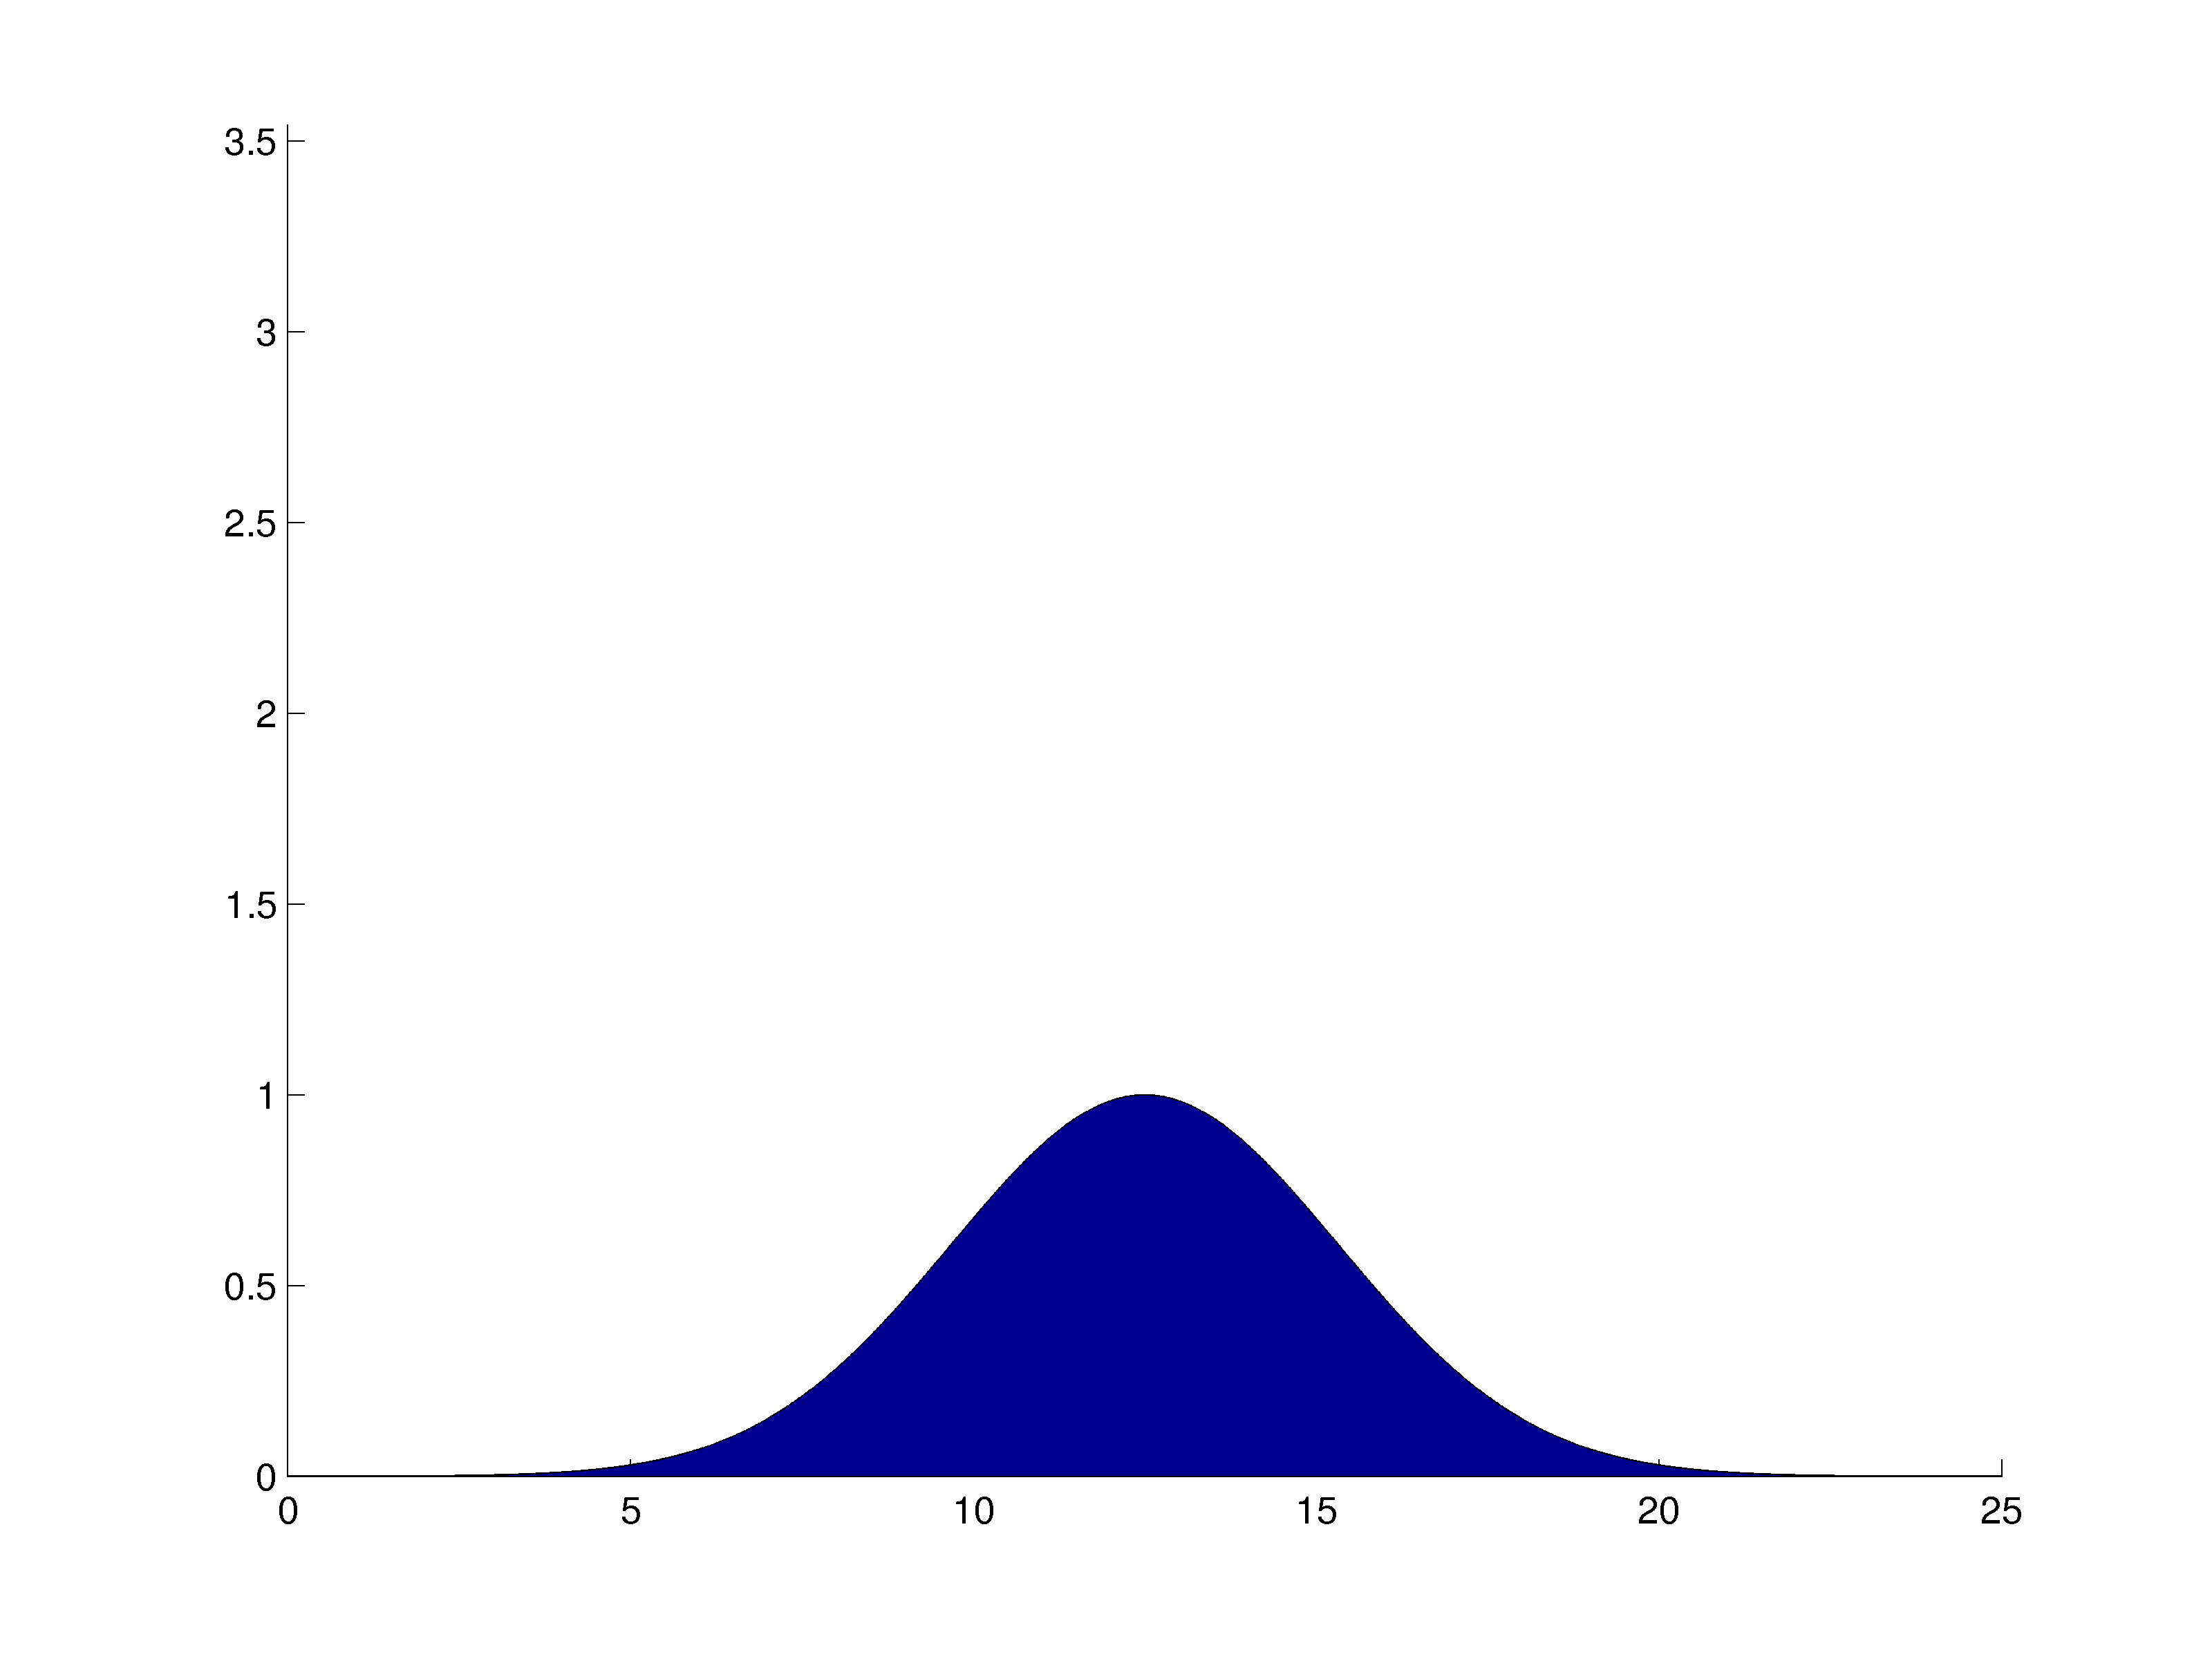
\includegraphics[width=\textwidth]{gfx/areainitial}
                \caption{Initial condition}
                \label{fig:area1}
\end{subfigure}
\begin{subfigure}[b]{0.49\textwidth}
                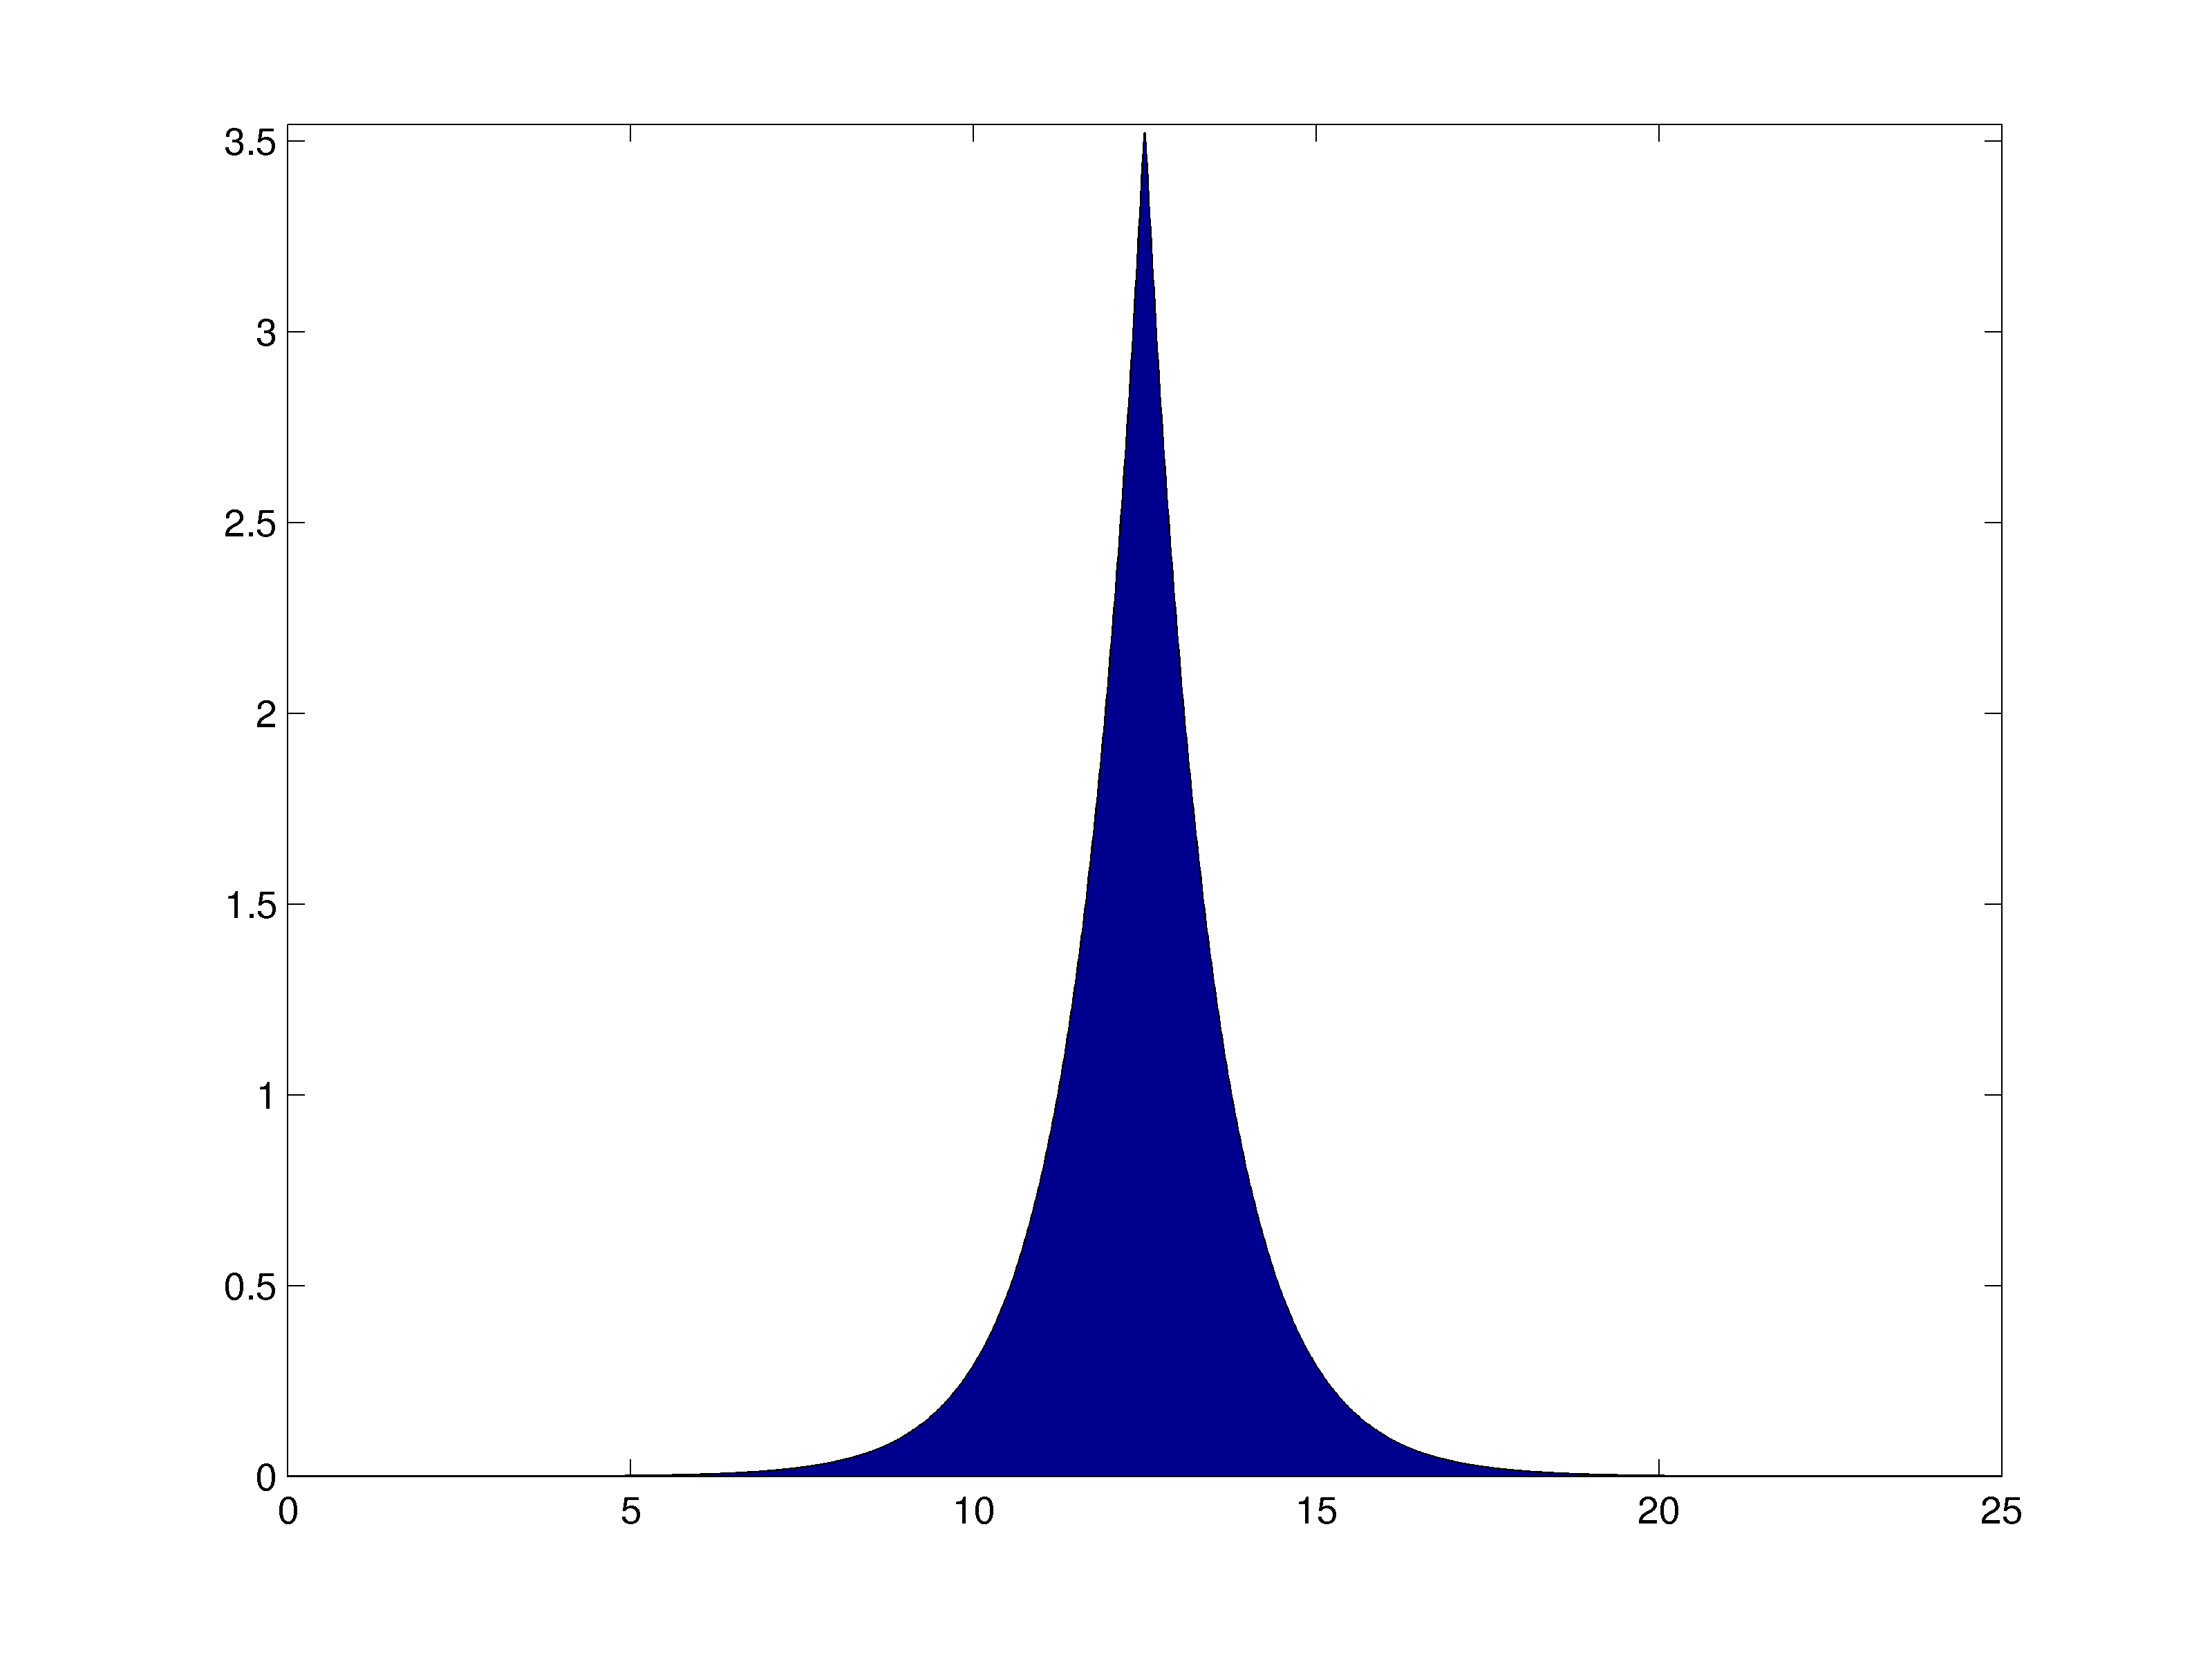
\includegraphics[width=\textwidth]{gfx/areapeakon}
                \caption{Peakon of same area}
                \label{fig:area2}
\end{subfigure}
\caption{Initial condition and peakon of same area, used to estimate $c$.}
\end{figure}


A preliminary conclusion based on the plot of errors for decreasing spacial stepsize $h$ (Figure \ref{fig:erroroftime}) shows that decreasing $h$ will improve the approximation. Figure \ref{fig:attimeT} shows that as the spacial stepsize $h$ decreases, our scheme becomes a good approximation of the solution. \\


Our numerical experiments show a rate of convergence in space which is slightly faster than a linear rate (Figure \ref{fig:loglog}). This was calculated using a short time interval, to reduce the effects of propagation of error. However, we experience that decreasing the temporal stepsize beyond a certain size increases the error. 

\begin{figure}[h]
        \centering
        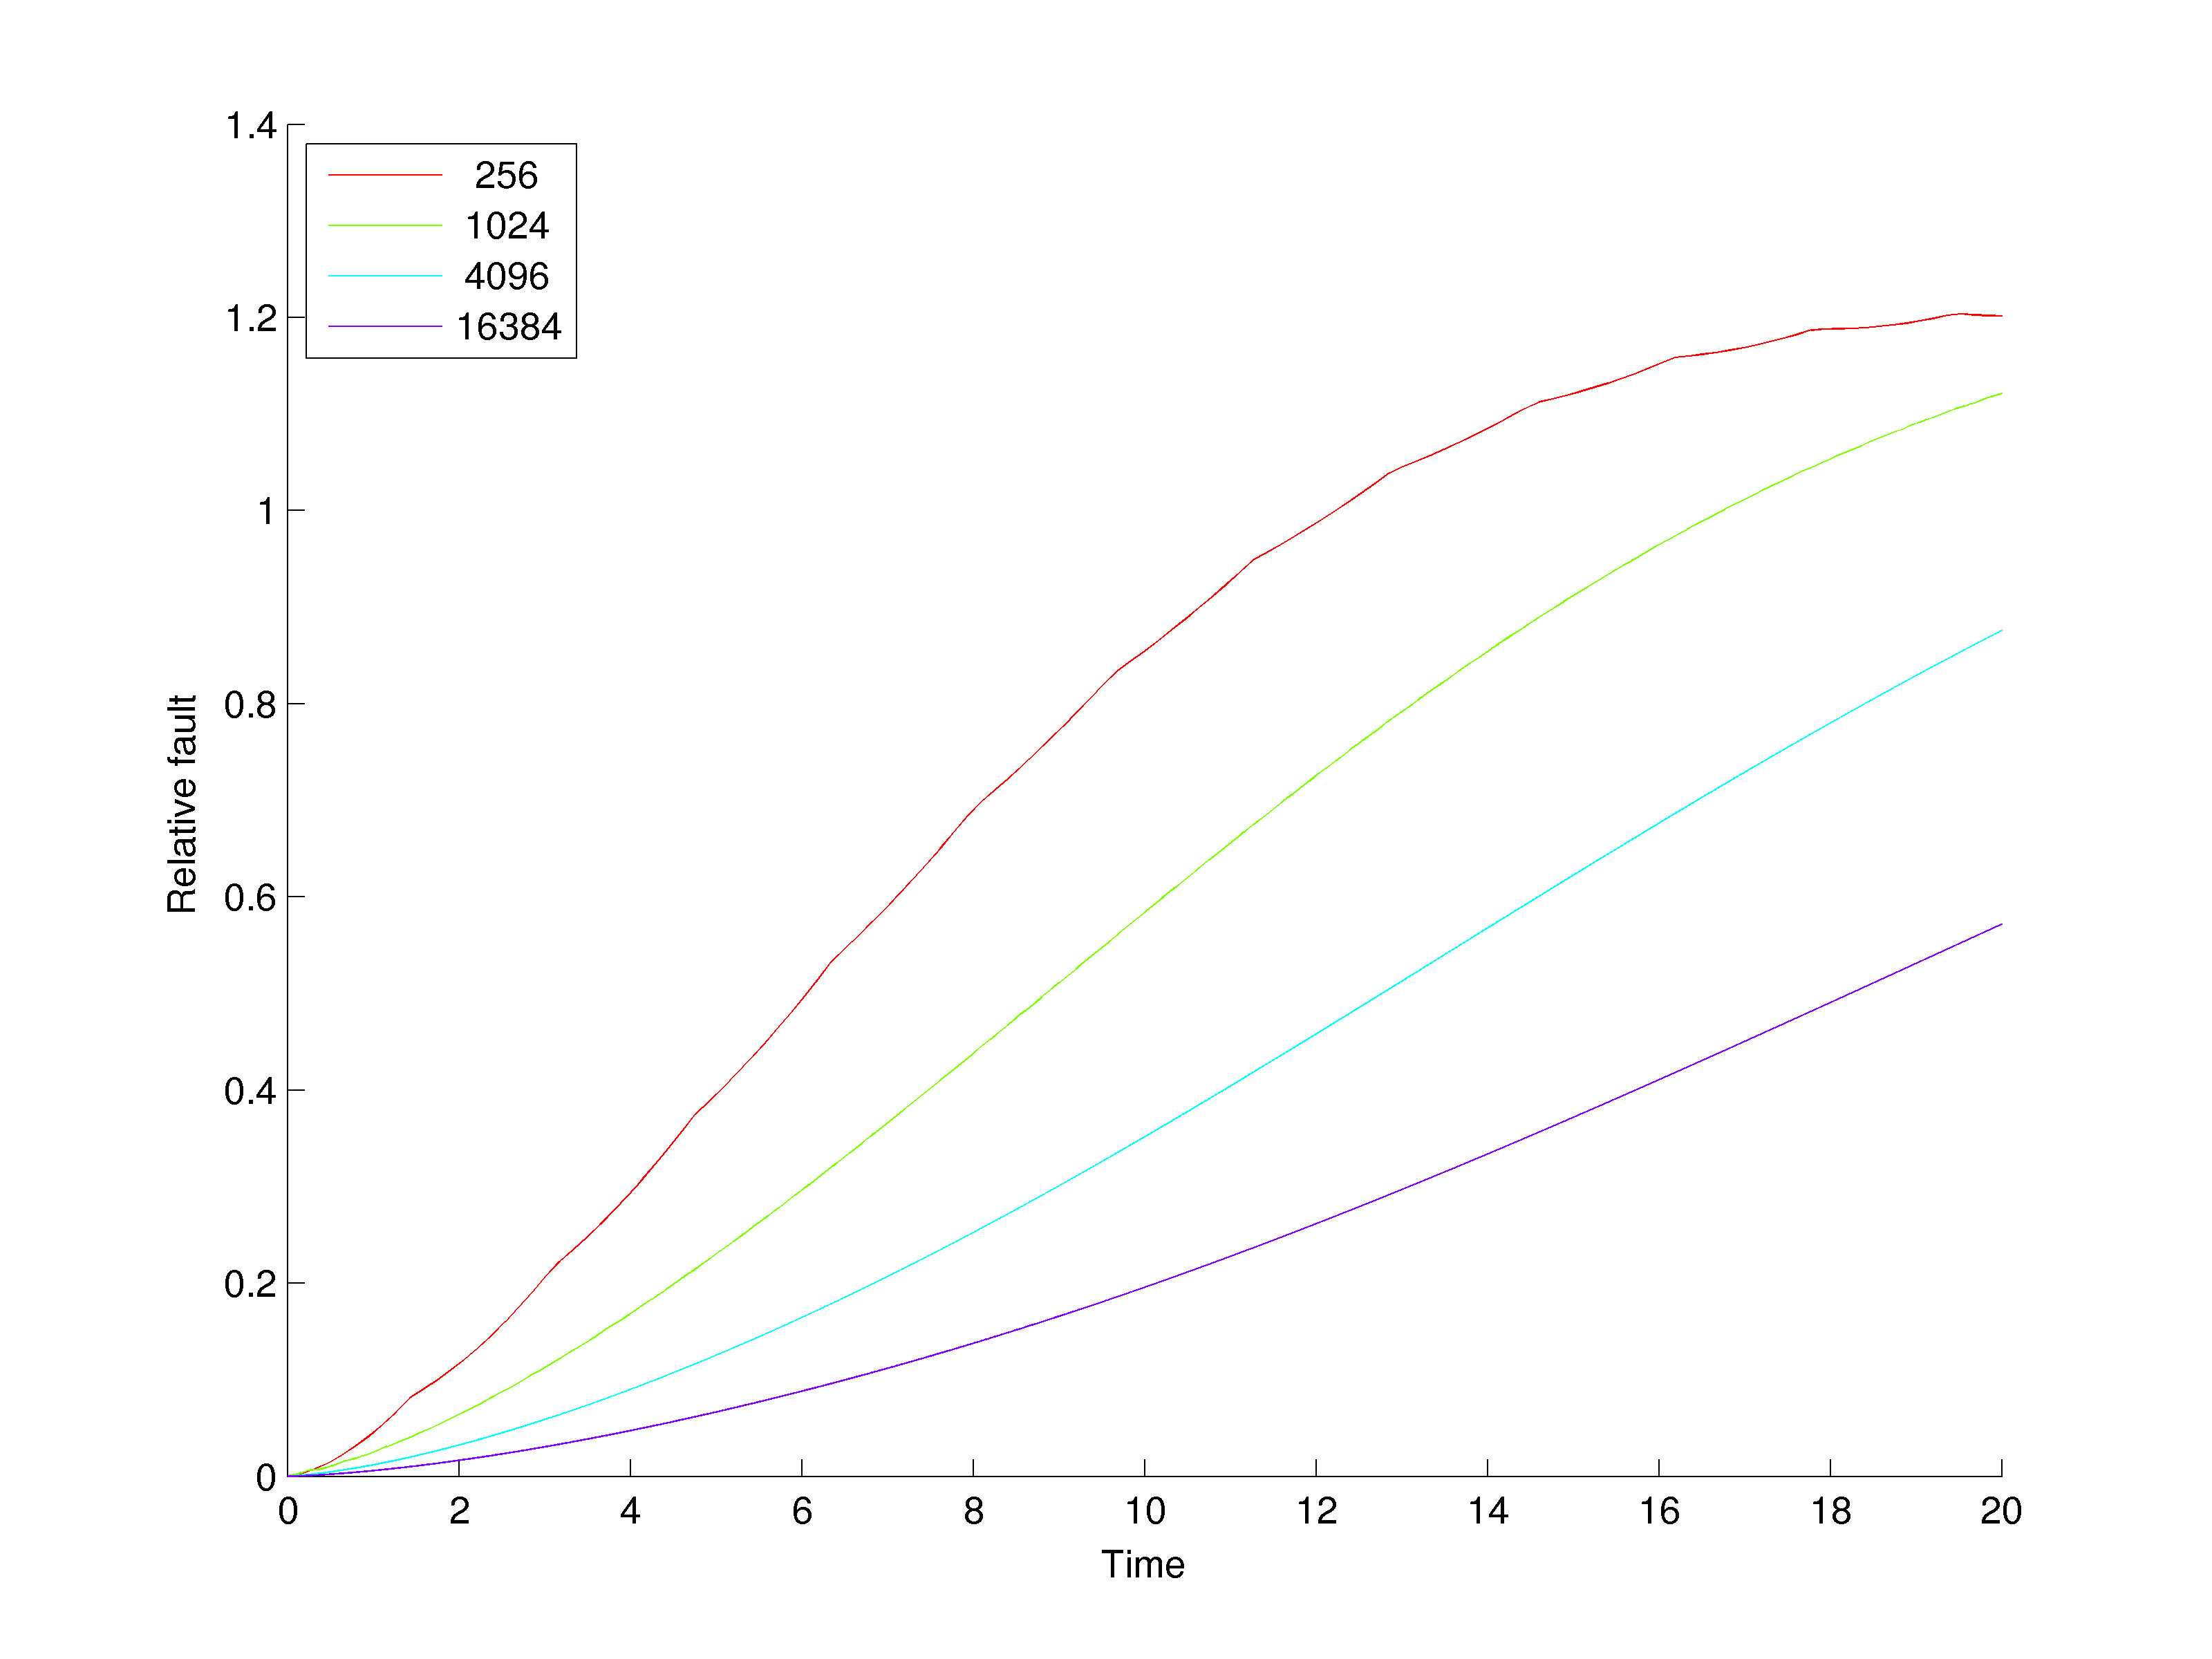
\includegraphics[width=0.8\textwidth]{gfx/erroroftime}
        \caption{Error plots for decreasing $h$, constant time and space interval.}
        \label{fig:erroroftime}
\end{figure}

\begin{figure}[h]
        \centering
        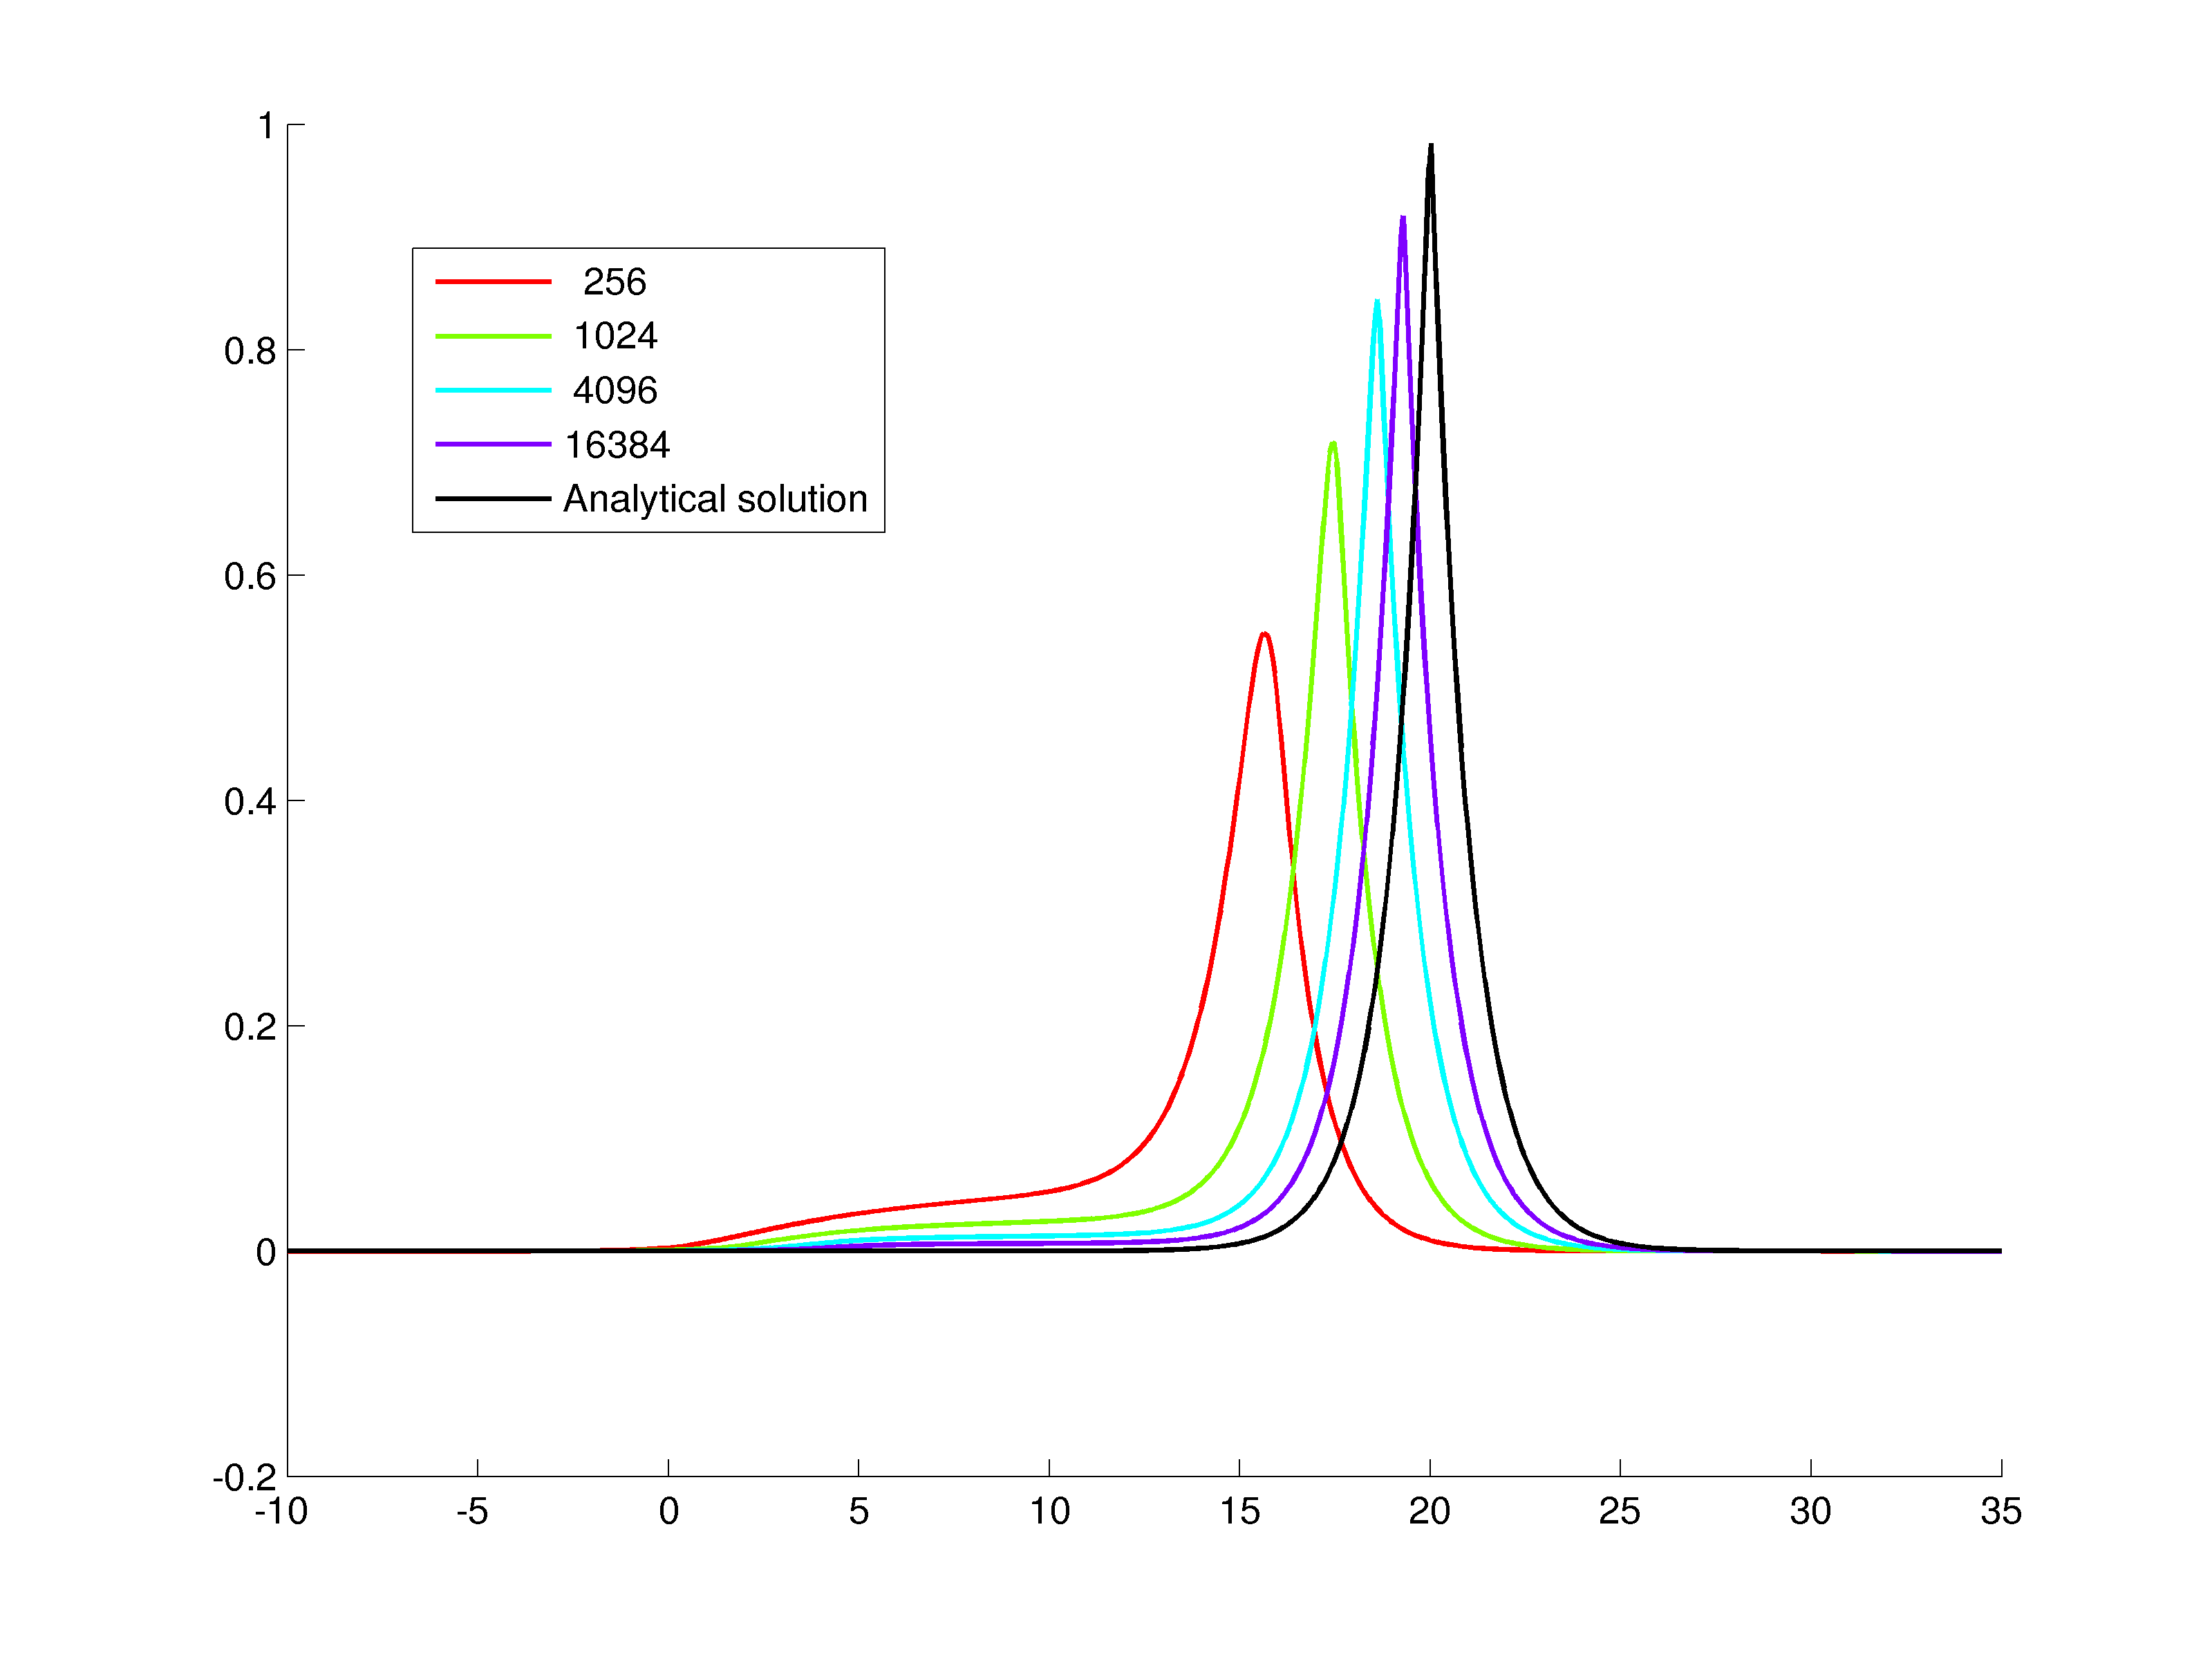
\includegraphics[width=0.8\textwidth]{gfx/attimeT}
        \caption{Plot of approximated solution together with analytical solution for decreasing spacial step $h$.}
        \label{fig:attimeT}
\end{figure}

\begin{figure}[h]
        \centering
        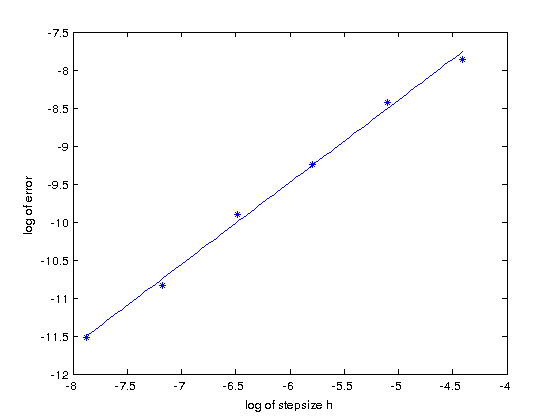
\includegraphics[width=0.8\textwidth]{gfx/loglog}
        \caption{Loglog plot - rate of convergence in space. In this plot, the red reference line has a slope of 1, while the blue line found through numerical experiments has a slope of 1.08}
        \label{fig:loglog}
\end{figure}

\subsection*{Semi-discretization}
Writing 
\begin{align*}
m_t = - D_- (m u) - m D u = f(m)
\end{align*},

one may obtain a system of ODEs which can be solved with standard numerical software, though each evaluation of $f$ requires a transformation from $m$ to $u$. Additionally, in the end one needs to transform the resulting matrix of $m$ values back to $u$. Testing a variety of MATLAB's builtin ODE solvers, including \emph{ode45}, \emph{ode15s} and \emph{ode113}, we surprisingly discovered that our explicit scheme based on Euler's method was far superior in every aspect to any other integrator available to us. 

The exact reason why is still unknown to us, though we suspect the discontinuous derivatives of the peakon solutions may cause problems for higher order schemes. This is at least consistent with the fact that the higher order schemes appear to smooth out the peaks of the solution.

Another interesting effect was observed when the timestep of the explicit scheme was decreased (below the bounded value given by our CFL condition) with the spatial step fixed. Numerical experiments suggest that the solution offered by the explicit scheme converges towards the solution of the higher order time integrators as the timestep goes towards zero. In other words, the increased error that results from too small timesteps is somehow bounded by the higher-order schemes. We have not yet been able to discover the cause, and our only hypothesis is at best a farfetched and unlikely guess: perhaps our scheme somehow possesses innate damping, which is inaccurately underestimated by Euler's method in such a way that the explicit scheme experiences less damping than the higher-order integrators?